\documentclass{MMCStyle}

% ---------- 常用包 ----------
\usepackage{zhlipsum,mwe}
\usepackage{lastpage}
\usepackage{setspace}
\usepackage{float}
\usepackage{longtable}
\usepackage{booktabs}
\usepackage{enumitem}
\usepackage{titlesec}
\usepackage{tabularx}
\usepackage{array}
\usepackage[table]{xcolor}

% ---------- 颜色 ----------
\definecolor{ReportTeal}{RGB}{24,156,196}
\definecolor{ReportStripe}{RGB}{231,239,246}

% ---------- 赛题信息 ----------
\bianhao{MC2604641}
\tihao{D}
\timu{三维装箱及多车型协同调度优化}
\keyword{三维装箱问题；启发式算法；异构货物约束；多车型调度；空间利用率优化}
\bibliographystyle{gbt7714-numerical}

% ---------- 全局排版 ----------
\setstretch{1.25}
\setcounter{tocdepth}{2}
\setlength{\parskip}{6pt plus 2pt minus 1pt}

% 标题间距
\titlespacing*{\section}{0pt}{1ex}{0.5ex}
\titlespacing*{\subsection}{0pt}{0.5ex}{0.2ex}
\titlespacing*{\subsubsection}{0pt}{0.4ex}{0.2ex}
\titlespacing*{\paragraph}{0pt}{0.5ex}{0.8em}

% 列表间距
\setlist[itemize]{itemsep=3pt, parsep=2pt, topsep=6pt, partopsep=2pt}
\setlist[enumerate]{itemsep=3pt, parsep=2pt, topsep=6pt, partopsep=2pt}

% 公式前后间距
\setlength{\abovedisplayskip}{10pt plus 2pt minus 5pt}
\setlength{\belowdisplayskip}{10pt plus 2pt minus 5pt}
\setlength{\abovedisplayshortskip}{6pt plus 2pt minus 3pt}
\setlength{\belowdisplayshortskip}{6pt plus 2pt minus 3pt}

% 页面边距
\geometry{left=2cm, right=2cm, top=2cm, bottom=2cm, footskip=1cm}

% 代码高亮（务必放在 \begin{document} 之前）
\usepackage{listings}
\usepackage{xcolor}

\definecolor{codebg}{RGB}{248,248,248}
\definecolor{codekw}{RGB}{0,70,140}
\definecolor{codestr}{RGB}{163,21,21}
\definecolor{codecom}{RGB}{0,128,0}
\definecolor{codenum}{RGB}{120,120,120}

\lstdefinestyle{pycolor}{
    language=Python,
    backgroundcolor=\color{codebg},
    basicstyle=\ttfamily\footnotesize,
    keywordstyle=\color{codekw}\bfseries,
    stringstyle=\color{codestr},
    commentstyle=\color{codecom}\itshape,
    numberstyle=\color{codenum}\scriptsize,
    numbers=left,
    numbersep=8pt,
    frame=single,
    framerule=0.3pt,
    breaklines=true,
    showstringspaces=false,
    tabsize=4
}

\begin{document}

	\begin{abstract}
	\setstretch{1.5}

本研究针对物流配送中的三维装箱与多车型协同调度问题。该问题受限于车厢空间和货物尺寸差异，加之易碎防压、定向放置、重心稳定、承重限制等复杂物理约束，构成典型的NP-Hard难题。这在快递电商、零担物流等行业中成为制约运输效率和降低成本的关键技术瓶颈。本课题建立基于混合整数规划的严谨数学模型，系统涵盖空间不重叠、载重、边界、方向与堆叠等多维度约束，设计融合极点搜索、动态贪心选择与多目标局部优化的高效启发式算法，实现秒级至分钟级求解。

问题一针对单车型装载优化，其核心挑战在于如何在多重物理约束下，同时最大化空间利用率和载重利用率。不同货物类型的尺寸、重量、易碎性差异巨大，传统的按体积或重量排序方法难以获得高质量方案。本算法采用多维度综合评分体系，系统考虑空间填充效率、结构稳定性和成本因素，对车型1和车型2分别实现了89.87\%和95.18\%的空间利用率以及53.53\%和73.44\%的载重利用率，接近理论上界。在3000件异构货物的测试上，分别仅需17辆车型1或8辆车型2完成全部运输，验证了算法的高效性。

问题二针对多车型协同调度，其主要困难在于如何在两个车型之间做出最优权衡决策。不同车型具有不同的容量、成本结构和装载特性，在"车辆数最少"与"成本最低"两种优化导向下可能产生不同结果。本研究通过全局优化框架，对所有可行方案进行系统评估。结果表明，在两种目标下均优选8辆车型2方案（总成本5600元），相比17辆车型1（总成本12600元）可节省车辆52.9\%、成本55.6\%。

为验证算法鲁棒性与泛化能力，进行了多维度敏感性分析与大规模数据测试。敏感性分析表明，算法对关键参数波动$\pm 20\%$保持高度稳定，在车辆成本、货物权重等变量变化时均能给出稳定方案，时间复杂度为O(n)。该方案为物流企业带来可量化效益-年运100批次可节省百万元级成本，车辆减少52.9\%显著降低碳排放，符合国家"双碳"战略。研究成果可广泛应用于快递电商、零担、冷链运输等领域。
\end{abstract}
    
	{\setstretch{1.5}  % 目录用单倍行距
	\tableofcontents}
	\newpage
	\clearpage
	\pagenumbering{arabic}
	\pagestyle{fancy}

\section{问题背景与研究意义}

\hspace{2em}降低全社会物流成本与培育“新质生产力”是我国“十五五”规划的核心战略要求。然而在实际物流配送场景中，受限于货车有限的空间，加之货物尺寸各异且面临易碎防压、放置方向、重心与承重限制等严苛的物理约束，使得三维装箱策略成为极具挑战的 NP-Hard 问题。为此，本课题立足于真实物流场景，通过构建严谨的数学规划模型与高效启发式算法，旨在微观层面攻克单车综合满载率最大化的技术堵点，并在宏观层面实现多车型调度下车队规模与总运输成本的最低化，最终为企业提供兼顾高装载率与经济效益的智慧化落地装箱方案。

\begin{figure}[H]
    \centering
    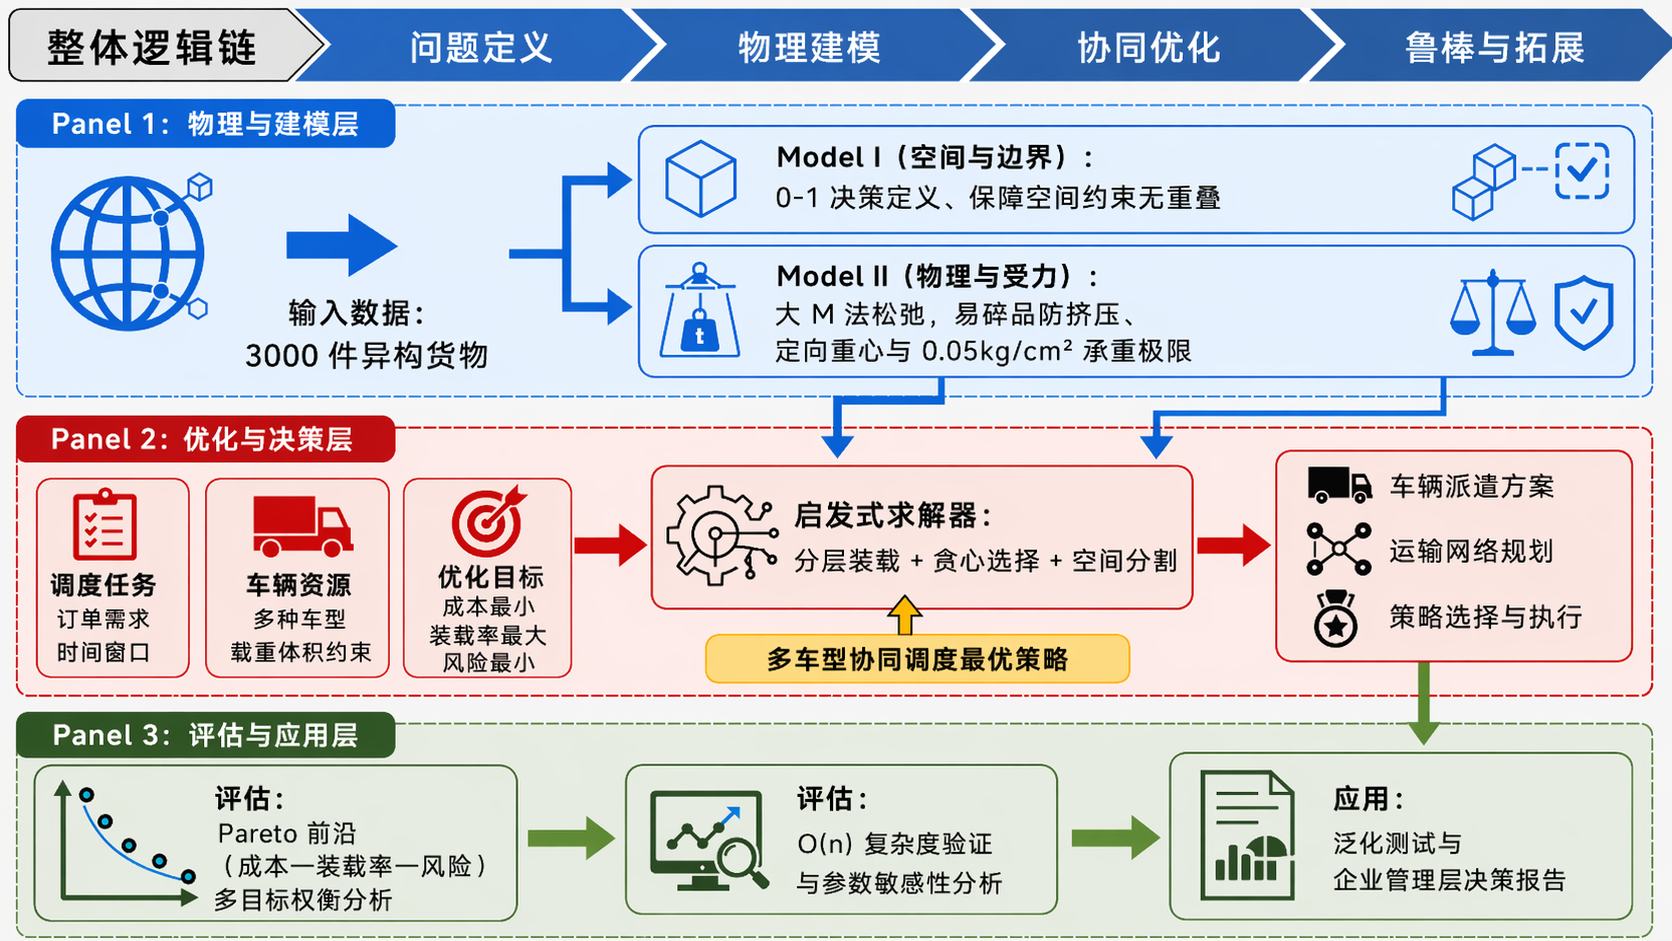
\includegraphics[width=0.88\textwidth]{流程图.png}
    \caption{课题研究思路与求解流程图}
    \label{fig:research_flowchart}
\end{figure}
\vspace{-1.6em}
\section{问题描述}


\begin{enumerate}[label=\arabic*., leftmargin=*]
    \item \textbf{问题一：短途单车型三维装箱策略优化}
    \begin{itemize}[leftmargin=*]
        \item \textbf{情景 A（极致单车满载）：} 分别以车型1和车型2为目标，从给定的货物集合中挑选货物，在严格遵守物理尺寸、载重极限、放置方向及复杂堆叠（如易碎防压、定向重心）等约束的前提下，建立三维装箱策略模型，以最大化单车的综合满载率（即同时兼顾“满容”与“满载”）。
        \item \textbf{情景 B（单一车型最少车辆）：} 若强制运完所有给定货物且仅允许使用一种车型，建立数学模型求解所需的理论最少车辆数。
        \item \textbf{算法与输出要求：} 设计并实现相应的三维装箱求解算法，输出包含每件货物在车厢相对坐标系中的空间三维坐标与姿态方向的具体装箱方案，并精确计算空间利用率与载重利用率。
    \end{itemize}
    
    \item \textbf{问题二：短途多车型组合配送优化}
    
    \hspace{2em}在同时开放车型1与车型2选用权限的条件下，要求制定将给定货物全部运完的全局调度与装箱组合方案。此问题包含两个优化的权衡方向：
    \begin{itemize}[leftmargin=*]
        \item \textbf{导向一（绝对数量最少）：} 建立以总运输车辆数最少为单一目标的装箱分配模型，并给出对应的配送方案。
        \item \textbf{导向二（经济成本最低）：} 考虑不同车型的单趟运输成本差异，建立以总运输成本最低为目标的优化方案，并深入对比分析两种不同导向对最终车队结构与装载策略产生的结果差异。
    \end{itemize}
    
    \item \textbf{问题三：管理层技术报告与算法鲁棒性验证}
    \begin{itemize}[leftmargin=*]
        \item \textbf{商业论证与敏感性分析：} 脱离纯粹的数学符号，撰写一份面向物流企业管理者的技术报告。需通俗、清晰地说明所构建模型与算法的核心机制，并针对关键参数进行敏感性分析，探讨其变动对装载率与运输总成本的边际影响。
        \item \textbf{泛化能力验证：} 基于更大规模的测试数据集，运行上述开发的求解程序，验证模型在应对海量货物时的求解效率与通用性，为企业的实际落地应用提供可靠的数据支撑。
    \end{itemize}
\end{enumerate}

\section{模型准备}
\subsection{坐标系建立与基本假设}

为准确描述货物在车厢内的空间位置与几何约束，本模型以车厢内部\textbf{右后下角}为坐标原点 $(0,0,0)$ 建立三维直角坐标系：

\begin{itemize}
\item \textbf{$X$ 轴}：沿车厢宽度方向，由右向左延伸。
\item \textbf{$Y$ 轴}：沿车厢长度方向，由后向前延伸。
\item \textbf{$Z$ 轴}：沿车厢高度方向，由下向上延伸。
\end{itemize}

五种货物类型的3D图例如下：
\begin{figure}[H]
    \centering
    
\includegraphics[width=1\linewidth]{figures/货物3D图例.png}
    \caption{货物图例}
    \label{fig:placeholder}
\end{figure}

\textbf{基本假设：}
\begin{enumerate}
\item 所有货物均为刚性长方体，装载过程中不发生形变。
\item 货物必须正交放置（即货物的边与车厢的边平行，不允许斜放）。
\item 不同货物的单位运输费用相同。
\item 假设定向件的方向为“向上”标识
\end{enumerate}

\subsection{符号说明}

\begin{longtable}{c c c p{8cm}}
\caption{核心数学符号说明表}\label{tab:symbols} \\
\toprule
\textbf{符号} & \textbf{分类} & \textbf{类型} & \textbf{物理含义说明（及单位）} \\
\midrule
\endfirsthead

\multicolumn{4}{c}{{\bfseries 表 \thetable\ -- 续表}} \\
\toprule
\textbf{符号} & \textbf{分类} & \textbf{类型} & \textbf{物理含义说明（及单位）} \\
\midrule
\endhead

\midrule
\multicolumn{4}{r}{{接下页 \dots}} \\
\endfoot

\bottomrule
\endlastfoot
$N$ & 集合 & - & 待装运货物总集合，$i,j\in N$ \\[2pt]
$N_{std}$ & 集合 & - & 标准件货物子集 \\[2pt]
$N_{fra}$ & 集合 & - & 易碎件货物子集 \\[2pt]
$N_{dir}$ & 集合 & - & 定向件货物子集 \\[2pt]
$k$ & 索引 & 整数 & 货物的正交摆放姿态编号，$k\in\{1,2,\dots,6\}$ \\[2pt]
$L,W,H$ & 参数 & 连续 & 车厢内部长度、宽度和高度，单位：cm \\[2pt]
$V$ & 参数 & 连续 & 车厢有效容积，单位：$\mathrm{cm^3}$ \\[2pt]
$M_{\max}$ & 参数 & 连续 & 车辆额定最大载重，单位：kg \\[2pt]
$P_{\max}$ & 参数 & 连续 & 货物承压极限，单位：$\mathrm{kg/cm^2}$ \\[2pt]
$l_i,w_i,h_i$ & 参数 & 连续 & 货物 $i$ 的原始长、宽、高，单位：cm \\[2pt]
$m_i,v_i$ & 参数 & 连续 & 货物 $i$ 的重量与体积 \\[2pt]
$D_{wk}$ & 参数 & 连续 & 货物在第 $k$ 种姿态下沿 $w\in\{x,y,z\}$ 方向的尺寸 \\[2pt]
$p_i$ & 变量 & 0-1 & 货物 $i$ 是否装入车厢 \\[2pt]
$x_i,y_i,z_i$ & 变量 & 连续 & 货物 $i$ 右后下角在车厢坐标系中的位置 \\[2pt]
$o_{ik}$ & 变量 & 0-1 & 货物 $i$ 是否采用第 $k$ 种摆放姿态 \\[2pt]
$s_{ix},s_{iy},s_{iz}$ & 变量 & 连续 & 货物 $i$ 装载后沿 $X,Y,Z$ 方向的实际占用尺寸 \\[2pt]
$sup_{ij}$ & 变量 & 0-1 & 货物 $j$ 是否对货物 $i$ 形成直接支撑 \\[2pt]
$Area_{ij}$ & 变量 & 连续 & 货物 $i$ 与货物 $j$ 在 $X$-$Y$ 平面的投影重叠面积 \\[2pt]
$M$ & 参数 & 连续 & 大 $M$ 法中的充分大常数 \\[2pt]

\end{longtable}

\section{短途单车型三维装箱策略优化模型}

\subsection{决策变量与约束条件}

 \hspace{2em}为准确描述货物在车厢内的装载状态、空间位置、摆放姿态及其相互支撑关系，本文将问题一中的单车型三维装箱模型统一表述为“变量定义 + 约束刻画”的整体框架。设待装货物集合为 $N$，车厢宽、长、高分别为 $W,L,H$，额定载重为 $M_{\max}$，则模型中的核心变量与约束如下。

\subsubsection{变量定义}

\noindent\textbf{1. 装载状态与空间坐标变量}

\begin{itemize}
\item \textbf{装载状态变量：}$p_i \in \{0,1\}, \quad \forall i \in N$

当货物 $i$ 被装入目标车厢时，$p_i=1$；否则 $p_i=0$。

\item \textbf{空间坐标变量：}$x_i,y_i,z_i \ge 0, \quad \forall i \in N$

表示货物 $i$ 被装入车厢后，其右后下角顶点在车厢坐标系中的三维坐标值，单位为 cm。
\end{itemize}

\noindent\textbf{2. 姿态与空间占用变量}

\begin{itemize}
\item \textbf{姿态选择变量：}$o_{ik} \in \{0,1\}, \quad \forall i \in N,\ \forall k \in \{1,2,\ldots,6\}$

表示货物 $i$ 是否采用第 $k$ 种正交摆放姿态。

\item \textbf{实际占用尺寸变量：}$s_{ix},s_{iy},s_{iz} > 0, \quad \forall i \in N$

分别表示货物 $i$ 在确定姿态后沿 $X,Y,Z$ 三个方向的实际占用长度。
\end{itemize}

\noindent\textbf{3. 空间相对位置变量}

\begin{itemize}
\item \textbf{方向相对指示变量：}$l_{ij},r_{ij},f_{ij},b_{ij},d_{ij},u_{ij} \in \{0,1\}, \quad \forall i,j \in N,\ i \neq j$

分别表示货物 $i$ 是否整体位于货物 $j$ 的左侧、右侧、前侧、后侧、下侧和上侧。
\end{itemize}

\noindent\textbf{4. 物理支撑与受力变量}

\begin{itemize}
\item \textbf{直接支撑变量：}$sup_{ij} \in \{0,1\}, \quad \forall i,j \in N,\ i \neq j$

表示货物 $j$ 是否对货物 $i$ 形成直接底部支撑。

\item \textbf{底部接地变量：}$c_i \in \{0,1\}, \quad \forall i \in N$

表示货物 $i$ 是否直接放置在车厢底板上。

\item \textbf{投影重叠面积变量：}$Area_{ij} \ge 0, \quad \forall i,j \in N,\ i \neq j$

表示货物 $i$ 与货物 $j$ 在 $X$-$Y$ 平面上的正投影重叠面积，用于描述支撑覆盖率与承压传递关系。
\end{itemize}

\subsubsection{约束描述}

\noindent\textbf{1. 载重与边界约束}

所有被装入车厢的货物总重量不得超过车辆额定载重，即
\begin{equation}
\sum_{i=1}^{n} p_i m_i \le M_{\max}.
\end{equation}

若货物 $i$ 被装入车厢，则其整体不能超出车厢边界，因此有
\begin{equation}
\left\{
\begin{aligned}
x_i+s_{ix}\le W\cdot p_i,\ \forall i\in N,\qquad
y_i+s_{iy}\le L\cdot p_i,\ \forall i\in N,\qquad
z_i+s_{iz}\le H\cdot p_i,\ \forall i\in N.
\end{aligned}
\right.
\end{equation}


\noindent\textbf{2. 三维不重叠约束}

若任意两件货物 $i$ 和 $j$ 均被装入车厢，则它们在三维空间中必须至少在一个方向上完全错开。利用大 $M$ 法可写为
\begin{equation}
\left\{
\begin{aligned}
x_i+s_{ix} &\le x_j+M(1-l_{ij}), &\quad
x_j+s_{jx} &\le x_i+M(1-r_{ij}),\\
y_i+s_{iy} &\le y_j+M(1-f_{ij}), &\quad
y_j+s_{jy} &\le y_i+M(1-b_{ij}),\\
z_i+s_{iz} &\le z_j+M(1-d_{ij}), &\quad
z_j+s_{jz} &\le z_i+M(1-u_{ij}).
\end{aligned}
\right.
\end{equation}

并满足
\begin{equation}
l_{ij}+r_{ij}+f_{ij}+b_{ij}+d_{ij}+u_{ij}\ge p_i+p_j-1,\quad \forall i,j\in N,\ i\neq j.
\end{equation}

\noindent\textbf{3. 姿态与方向约束}

任何长方体货物均可在正交姿态集合中选择放置方式。若第 $k$ 种姿态下货物沿 $w \in \{x,y,z\}$ 方向的映射尺寸为 $D_{wk}$，则有
\begin{equation}
s_{iw}=\sum_{k=1}^{6} o_{ik} D_{wk}, \quad w \in \{x,y,z\}.
\end{equation}

对于标准件和易碎件，可任选正交姿态，因此满足
\begin{equation}
\sum_{k=1}^{6} o_{ik}=p_i, \quad \forall i \in N_{std}\cup N_{fra}.
\end{equation}

对于定向件，仅允许采用题目规定姿态，因此有
\begin{equation}
o_{i1}=p_i,\qquad \sum_{k=2}^{6} o_{ik}=0,\quad \forall i \in N_{dir}.
\end{equation}

\noindent\textbf{4. 易碎件防压与全支撑约束}

易碎件 $i \in N_{fra}$ 的上方绝对不能再放置其他货物。若其与任意货物 $j$ 在 $X$-$Y$ 平面上存在重叠，则只能满足“$j$ 在其下方”的关系，即
\begin{equation}
l_{ij}+r_{ij}+f_{ij}+b_{ij}+u_{ij}\ge p_i+p_j-1,\quad \forall i \in N_{fra},\ \forall j \in N,\ i\neq j.
\end{equation}

同时，若易碎件不直接落地，则其底面必须由下方标准件实现全支撑，因此有
\begin{equation}
\sum_{j \in N_{std}} Area_{ij}\cdot sup_{ij} \ge s_{ix}s_{iy}-M(1-p_i)-Mc_i,\quad \forall i \in N_{fra}.
\end{equation}

\noindent\textbf{5. 定向件重心稳定约束}

若定向件 $i \in N_{dir}$ 被放置在货物 $j$ 上方，则其底面几何中心必须落在支撑货物的投影范围内，故有
\begin{equation}
\left\{
\begin{aligned}
&x_i+0.5s_{ix}\ge x_j-M(1-sup_{ij}),\\
&x_i+0.5s_{ix}\le x_j+s_{jx}+M(1-sup_{ij}),\\
&y_i+0.5s_{iy}\ge y_j-M(1-sup_{ij}),\\
&y_i+0.5s_{iy}\le y_j+s_{jy}+M(1-sup_{ij}),\\
&\forall i \in N_{dir},\ \forall j \in N,\ i \neq j.
\end{aligned}
\right.
\end{equation}

\noindent\textbf{6. 承重约束}

题目规定货物承压极限为 $500 \text{kg/m}^2$，换算为
\begin{equation}
P_{\max}=0.05\ \text{kg/cm}^2.
\end{equation}

因此，对任意被装入车厢的货物 $j$，其承受的来自上方货物的累计压强必须满足
\begin{equation}
\sum_{i \in N,\ i \neq j}\left(m_i \cdot \frac{Area_{ij}}{s_{ix}s_{iy}} \cdot u_{ij}\right)
\le P_{\max}\cdot (s_{jx}s_{jy}) + M(1-p_j),\quad \forall j \in N.
\end{equation}

\noindent\textbf{7. 顶部安全间隙约束}

为保证运输安全，顶层货物与车厢顶部之间至少保留 3 cm 安全间隙，因此车厢有效高度满足
\begin{equation}
z_i+s_{iz}\le (H-3)\cdot p_i,\quad \forall i \in N.
\end{equation}
\vspace{-2em}
\begin{figure}[H]
    \centering   
\includegraphics[width=0.8\textwidth]{figures/约束.png}
    \caption{问题一主要装箱约束示意图}
    \label{fig:problem1_constraints}
\end{figure}
\vspace{-1em}
综上，上述变量与约束共同构成了问题一单车型三维装箱模型的数学基础：变量部分刻画“装不装、怎么放、谁支撑谁”，约束部分则保证装箱方案在几何上可行、在物理上稳定、在工程上可执行，从而为后续情景 A 与情景 B 的求解算法提供统一的建模支撑。


\subsection{情景 A：单车满载率最大化}

情景 A 的目标是在给定车型下，从附件 1 的货物集合中选择合适货物装入单辆车厢，并在满足边界、非重叠、承压、易碎件全支撑、定向件姿态与重心稳定等约束的前提下，使单车综合满载率最大。本文将体积利用率与载重利用率按等权组合，建立目标函数
\begin{equation}
\max Z_A=\alpha \eta_v+\beta \eta_w,
\end{equation}
其中
\begin{equation}
\eta_v=\frac{\sum_i p_i v_i}{V},\qquad
\eta_w=\frac{\sum_i p_i m_i}{M_{\max}},\qquad
\alpha=\beta=0.5.
\end{equation}

在实现层面，车型1采用极点启发式装箱，并增加顶层 $G2$ 局部重装修复；车型2采用高密度单车装箱结果。

\paragraph{求解步骤}
为使建模与程序实现保持一致，单车求解过程可概括为以下四步：
\begin{enumerate}
    \item \textbf{货物候选生成与排序：} 按货物类别、尺寸规则性和堆叠约束对候选货物进行排序，优先考虑对整体结构更稳定、空间填充更充分的货物组合。
    \item \textbf{极点搜索与姿态遍历：} 在车厢内动态维护可放置极点集合，对每个候选货物遍历允许姿态，并优先选择贴底、贴边、支撑充分的放置方式。
    \item \textbf{可行性检验：} 对每次放置同时进行边界、重叠、支撑率、承压、易碎件不可受压以及定向件重心投影等约束校验。
    \item \textbf{结果筛选与局部修复：} 对不同策略得到的可行装箱方案计算综合满载率，保留最优解。
\end{enumerate}

\begin{figure}[H]
    \centering
    
\includegraphics[width=0.7\textwidth]{figures/sceneA_metrics_compare.png}
    \caption{情景 A 两种车型关键指标对比图}
    \label{fig:sceneA_metrics_compare}
\end{figure}

根据程序输出的汇总文件与装箱结果，情景 A 的最优单车方案如表 \ref{tab:single_truck_result_new} 所示。可以看出，车型2在空间利用率、载重利用率和综合满载率三个维度上均优于车型1。

\begin{table}[H]
\centering
\caption{情景 A 单车满载率最大化求解结果}
\label{tab:single_truck_result_new}
\renewcommand{\arraystretch}{1.25}
\setlength{\tabcolsep}{7pt}
\small
\begin{tabular}{ccccccc}
\rowcolor{ReportTeal}
\color{white}\textbf{车型} &
\color{white}\textbf{装载货物数} &
\color{white}\textbf{总体积 (cm$^3$)} &
\color{white}\textbf{总重量 (kg)} &
\color{white}\textbf{空间利用率} &
\color{white}\textbf{载重利用率} &
\color{white}\textbf{综合满载率} \\
\rowcolor{white}
车型1 & 214件 & 17,200,000 & 3,212 & 89.87\% & 53.53\% & 71.70\% \\
\rowcolor{ReportStripe}
车型2 & 408件 & 39,168,000 & 7,344 & 95.18\% & 73.44\% & 84.31\% \\
\end{tabular}
\end{table}


\paragraph{车型1装箱结果分析}
车型1的当前最优单车方案共装入 214 件货物，具体构成为 $G2\times64$ 与 $G5\times150$。从装箱结构上看，该方案采用了“底部定向件规则铺底，上部标准件均匀补齐”的思路：大量 $G5$ 在底层形成连续平台，保证了承压稳定性与底部空间的高效利用；$G2$ 由于尺寸更小、摆放更灵活，被集中布置在上层用于修补顶部剩余空间。该方案的空间利用率达到 89.87\%，载重利用率达到 53.53\%，说明车型1在有限长度条件下已经形成了较为紧凑的“厚平台 + 顶部补缝”式结构。

\begin{figure}[H]
    \centering
    
\includegraphics[width=0.86\textwidth]{figures/legacy_1.png}
    \caption{车型1单车三维装箱分层图}
    \label{fig:truck1_3d}
\end{figure}

从三视图进一步观察可知，车型1的俯视图几乎被规则阵列完全覆盖，说明底层排布已经接近满铺；正视图与侧视图则表明，车厢下部主要由 $G5$ 构成高稳定平台，而顶部留出的薄层空间被 $G2$ 有效填充，这正是车型1能够在较小车厢中继续提高空间利用率的关键。

\begin{figure}[H]
    \centering
    
\includegraphics[width=0.92\textwidth]{figures/legacy_fig4_type1_views.png}
    \caption{车型1单车三视图}
    \label{fig:truck1_views}
\end{figure}

平面热力图进一步说明了车型1方案的占用特点：热区主要集中在规则网格交汇位置，说明算法在搜索过程中更倾向于形成均匀、连续的支撑骨架；中间和边缘位置的颜色分布较为均衡，表明该方案并非局部堆积，而是整体性较强的高密度铺排结构。
\vspace{-2.6em}
\begin{figure}[H]
    \centering
    
\includegraphics[width=0.65\textwidth]{figures/sceneA_type1_heatmap.png}
    \caption{车型1平面占用热力图}
    \label{fig:truck1_heatmap}
\end{figure}
\vspace{-1.6em}
\paragraph{车型2装箱结果分析}
车型2的当前最优单车方案共装入 408 件货物，全部为定向件 $G5$。这说明在车型2更大的车厢尺度下，程序判定“直接使用单一规则货物形成整车高密度铺排”比混装更优。由于 $G5$ 的几何尺寸与车型2的车厢宽度、长度和高度匹配度很高，算法可以在底层快速形成高度规则的阵列，并持续向上堆叠，最终得到极为接近满容状态的单车方案。其空间利用率达到 95.18\%，载重利用率达到 73.44\%，显著高于车型1。

\begin{figure}[H]
    \centering
    
\includegraphics[width=0.86\textwidth]{figures/legacy_2.jpg}
    \caption{车型2单车三维装箱分层图}
    \label{fig:truck2_3d}
\end{figure}
\vspace{-1.6em}
车型2的三视图显示出非常鲜明的“规则满铺”特征：俯视图、正视图和侧视图均接近整块矩形区域，说明该方案的边角损失极小，车厢长宽高三个方向都被充分利用。与车型1相比，车型2并没有明显的局部补缝结构，而是更接近于理想的整车规则堆叠状态，因此综合满载率明显更高。

\begin{figure}[H]
    \centering
    
\includegraphics[width=0.92\textwidth]{figures/legacy_fig5_type2_views.png}
    \caption{车型2单车三视图}
    \label{fig:truck2_views}
\end{figure}

车型2的热力图也验证了这一结论：高占用区域沿车厢平面均匀分布，热区呈现连续且规则的条带状结构，说明该方案在空间利用上更接近整体最优，而不是依赖局部修补。正因如此，车型2不仅体积利用率更高，其重量利用率也同步提升，体现出更强的单车装载能力。

\begin{figure}[H]
    \centering
    
\includegraphics[width=0.65\textwidth]{figures/sceneA_type2_heatmap.png}
    \caption{车型2平面占用热力图}
    \label{fig:truck2_heatmap}
\end{figure}
\paragraph{情景 A 结论}
综合来看，车型1的优势在于能够通过“平台构建 + 顶层补缝”形成较高的空间利用率，而车型2则依赖更优的尺度匹配关系，实现近似整车满铺的高密度装载。按 $\alpha=\beta=0.5$ 计算，车型1的综合满载率为 71.70\%，车型2达到 84.31\%。因此，在情景 A 的单车满载率最大化目标下，车型2对应的单车装箱方案整体表现更优。


\subsection{情景 B：单一车型最少车辆数}

\hspace{2em}在情景 B 中，要求将附件 1 中扩充后的全部 3000 件货物一次性运输完毕，且运输过程中只允许使用同一种车型。与情景 A 的“单车综合满载率最大化”不同，本问的优化目标变为：在满足尺寸、载重、姿态、堆叠、承压、易碎防压和定向件稳定性等全部工程约束的前提下，使所需车辆总数最少。本文采用“\textbf{单车可行装箱 + 逐车递增调度}”的两层求解框架。

\paragraph{1. 求解思路}
固定某一车型后，程序按照如下步骤求解最少车辆数：
\begin{enumerate}
    \item \textbf{计算理论下界。} 由全部货物总体积和总重量，分别计算体积下界与载重下界，并取两者较大值作为该车型的理论最少车辆数。
    \item \textbf{构造剩余货物集合。} 初始时将全部 3000 件货物纳入待装集合；每完成一辆车的装箱后，从剩余集合中扣除已装货物。
    \item \textbf{执行单车装箱。} 对当前剩余货物，调用多策略极点装箱器，对“货物-姿态-极点”组合依次进行边界、重叠、支撑率、承压、易碎件禁压和定向件重心投影检验，并保留当前车辆的最优可行解。
    \item \textbf{逐车递增调度。} 若仍有货物未装完，则启用下一辆同型号车辆，重复单车装箱过程，直到全部货物被分配完成。
    \item \textbf{汇总车队结果。} 对两种车型分别统计实际车辆数、总运输成本、车队空间利用率与车队载重利用率，并据此比较优劣。
\end{enumerate}

\paragraph{2. 结果汇总}
设全部货物总体积和总重量分别为
\begin{equation}
V_{\mathrm{tot}}=287{,}350{,}000\ \mathrm{cm^3},\qquad
M_{\mathrm{tot}}=41{,}100\ \mathrm{kg}.
\end{equation}
若固定采用车型 $r$，则理论下界可写为
\begin{equation}
N_r^{\mathrm{LB}}=\max\left\{
\left\lceil \frac{V_{\mathrm{tot}}}{V_r}\right\rceil,
\left\lceil \frac{M_{\mathrm{tot}}}{M_r}\right\rceil
\right\}.
\end{equation}
\vspace{-1.6em}
\begin{table}[H]
\centering
\caption{单一车型最少车辆数求解结果}
\label{tab:min_trucks_new}
\renewcommand{\arraystretch}{1.25}
\setlength{\tabcolsep}{8pt}
\small
\begin{tabular}{cccccc}
\rowcolor{ReportTeal}
\color{white}\textbf{车型} &
\color{white}\textbf{理论下界} &
\color{white}\textbf{实际车辆数} &
\color{white}\textbf{总运输成本（元）} &
\color{white}\textbf{车队空间利用率} &
\color{white}\textbf{车队载重利用率} \\
\rowcolor{white}
车型1 & 16辆 & 17辆 & 7650 & 88.31\% & 40.29\% \\
\rowcolor{ReportStripe}
车型2 & 7辆 & 8辆 & 5600 & 87.29\% & 51.38\% \\
\end{tabular}
\end{table}
\vspace{-1.6em}

从表 \ref{tab:min_trucks_new} 可以看出，两种车型的实际结果都只比理论下界多 1 辆，说明当前“逐车递增 + 单车最优装箱”框架已经较接近可实现的最优水平。
\paragraph{3. 车型 1 方案分析}
车型 1 的车厢尺度相对较小，因此在处理 3000 件异构货物时更容易出现尾部碎片空间。程序运行结果表明，车型 1 共需 17 辆车，其中前 9 辆车的装箱结构高度一致，基本形成了稳定重复的“主力模板”。这说明在前期货物类型较完整时，算法能够持续输出较为规整的高质量排布方案。对应代表性结果如图\ref{fig:placeholder} 所示。
\begin{figure}[H]
    \centering    
\includegraphics[width=0.35\linewidth]{figures/3.png}
    \caption{车型 1 前 9 辆车的代表性装箱方案}
    \label{fig:placeholder}
\end{figure}

\begin{figure}
    \centering
    
\includegraphics[width=0.8\textwidth]{figures/2.jpg}
    \caption{车型1后16辆车的收尾装箱方案}
    \label{fig:type1_tail_plan}
\end{figure}


随着剩余货物结构逐步变得不规则，后续 8 辆车更多承担“收尾装载”和“局部补齐”任务，其空间结构明显不同于前期主力模板。此时，算法需要在有限车厢内处理更多不规则剩余件，因此局部空隙和层间补缝现象会更加突出。车型 1 后续车辆的装箱结果如图 \ref{fig:type1_tail_plan} 所示。


综合来看，车型 1 虽然能够完成全部货物的运输任务，但由于小车厢在后期更容易产生碎片化空间，最终需要 17 辆车才能完成全部装运。

\paragraph{4. 车型 2 方案分析}
车型 2 具有更大的长度、宽度和有效容积，因此单车内部具有更强的排布自由度。程序结果显示，车型 2 仅需 8 辆车即可完成全部货物运输。相比车型 1，车型 2 在大体量装载场景下更容易形成连续的大块堆叠区，从而降低尾部残余货物对整体调度的不利影响。车型 2 的整体装箱结果如图 \ref{fig:type2_all_plan} 所示。

\begin{figure}[H]
    \centering
    
\includegraphics[width=0.88\textwidth]{figures/1.jpg}
    \caption{车型2共 8 辆车的装箱结果总览}
    \label{fig:type2_all_plan}
\end{figure}

由图 \ref{fig:type2_all_plan} 看出，车型 2 在多数车辆中都保持了较好的层状连续性和排布特征。虽然从车队整体空间利用率看，车型 2 与车型 1 相差不大，但车型 2 的车队载重利用率更高、总车辆数更少，因此在实际调度中可以显著降低总运输成本。两种车型的详细统计参数如图\ref{fig:placeholder111}所示。

\begin{figure}[H]
    \centering
    
\includegraphics[width=0.9\linewidth]{figures/单一车型结果统计拼图.jpg}
    \caption{单一车型结果统计拼图}
    \label{fig:placeholder111}
\end{figure}

\paragraph{5. 装箱方案输出}
程序为每辆车自动生成可执行的装箱明细文件，输出内容包括：货物编号 \texttt{item\_id}、货物类型 \texttt{cargo\_type}、右后下角三维坐标 $(x,y,z)$、实际占用尺寸 $(dx,dy,dz)$ 以及货物重量 \texttt{weight}。这些坐标级结果可直接用于三维可视化展示，也可直接作为现场装车的执行参考。

\paragraph{6. 本问结论}
综上，在问题一第二小问中，固定车型条件下的最少车辆数求解结果为：车型 1 需要 17 辆，车型 2 需要 8 辆。两种车型的结果都仅比理论下界多 1 辆，说明当前启发式装箱与逐车调度算法具有较好的求解质量。由于车型 2 能够以更少的车辆完成全部运输任务，且总运输成本更低，因此在本题的单一车型约束下，应优先选择车型 2 作为最优运输方案。

\section{短途多车型组合配送优化模型}

\subsection{变量定义与约束条件}

问题二在问题一单车三维装箱模型的基础上，进一步引入车型选择与多车协同调度决策。设车型集合为
\begin{equation}
K=\{1,2\},
\end{equation}
其中车型1和车型2的有效容积、额定载重和单次运输成本分别记为 $(V_k,M_k,C_k)$。根据题目数据与程序参数，
\begin{equation}
V_1=19.1394\ \mathrm{m^3},\quad M_1=6000\ \mathrm{kg},\quad C_1=450\ \mathrm{元},
\end{equation}
\begin{equation}
V_2=41.1502\ \mathrm{m^3},\quad M_2=10000\ \mathrm{kg},\quad C_2=700\ \mathrm{元}.
\end{equation}
设 $v\in\{1,2,\dots,V_{\max}\}$ 为车辆编号，$i\in N$ 为货物编号，则问题二新增如下决策变量：

\begin{equation}
y_{kv}\in\{0,1\},
\end{equation}
其中 $y_{kv}=1$ 表示启用第 $k$ 种车型的第 $v$ 辆车，$y_{kv}=0$ 表示不启用；
\begin{equation}
p_{ikv}\in\{0,1\},
\end{equation}
其中 $p_{ikv}=1$ 表示货物 $i$ 被分配至第 $k$ 种车型的第 $v$ 辆车中，$p_{ikv}=0$ 表示未被分配至该车。

除上述全局调度变量外，问题一中的单车装箱变量（如坐标变量 $(x_i,y_i,z_i)$、姿态变量 $o_{ik}$、支撑变量 $sup_{ij}$ 等）在问题二中仍然逐车成立，只是其适用对象由“单辆车内的货物集合”扩展为“每一辆已启用车辆所承载的货物子集”。

问题二需同时满足以下约束。

\paragraph{1. 货物完备性约束}
所有货物必须且只能被分配到唯一一辆已启用车辆中，即
\begin{equation}
\sum_{k\in K}\sum_{v=1}^{V_{\max}}p_{ikv}=1,\qquad \forall i\in N.
\end{equation}

\paragraph{2. 逻辑指派约束}
若某车辆未启用，则不能向其中分配货物，因此有
\begin{equation}
p_{ikv}\le y_{kv},\qquad \forall i\in N,\ \forall k\in K,\ \forall v.
\end{equation}

\paragraph{3. 单车重量约束}
对任意已启用车辆，其内部货物总重不得超过对应车型的额定载重，即
\begin{equation}
\sum_{i\in N}p_{ikv}m_i\le M_k\,y_{kv},\qquad \forall k\in K,\ \forall v.
\end{equation}

\paragraph{4. 单车几何与工程约束}
对于任意已启用车辆 $(k,v)$，其内部货物必须逐车满足问题一中的全部单车装箱约束。

因此，问题二本质上是“外层车型--车辆分配”与“内层单车三维装箱”的耦合优化问题。结合程序实现，本文采用 \texttt{packing\_utils.py} 提供单车装箱与可行性校验，由 \texttt{q12.py} 完成多车调度与结果汇总，并使用 \texttt{packer.py} 输出代表性方案图。

\subsection{情景 A：总运输车辆数最少}

情景 A 的目标是在同时允许使用两种车型的条件下，使运输全部 3000 件货物所需的车辆总数最少。其目标函数为
\begin{equation}
\min Z_A=\sum_{k\in K}\sum_{v=1}^{V_{\max}}y_{kv}.
\end{equation}

\paragraph{1. 理论下界分析}

设总货物体积与总重量分别为
\[
V_{\mathrm{tot}}=287{,}350{,}000\ \mathrm{cm}^3,\qquad
W_{\mathrm{tot}}=41{,}100\ \mathrm{kg}.
\]
在考虑车厢顶部安全间隙后，采用有效高度 $H_{\mathrm{eff}}$ 计算单车有效容积。记第 $k$ 类车辆单车有效容积为 $C_k$、最大载重为 $Q_k$，则车辆数理论下界为
\[
N_{\mathrm{LB}}(k)=\max\!\left(
\left\lceil \frac{V_{\mathrm{tot}}}{C_k}\right\rceil,\ 
\left\lceil \frac{W_{\mathrm{tot}}}{Q_k}\right\rceil
\right).
\]

\paragraph{车型2（大车）}
\[
C_2=680\times245\times247=41{,}150{,}200\ \mathrm{cm}^3,\qquad Q_2=10{,}000\ \mathrm{kg},
\]
\[
\left\lceil \frac{V_{\mathrm{tot}}}{C_2}\right\rceil
=\left\lceil \frac{287{,}350{,}000}{41{,}150{,}200}\right\rceil=7,\qquad
\left\lceil \frac{W_{\mathrm{tot}}}{Q_2}\right\rceil
=\left\lceil \frac{41{,}100}{10{,}000}\right\rceil=5.
\]
因此
\[
N_{\mathrm{LB}}(\mathrm{Type2})=\max(7,5)=7.
\]

\paragraph{车型1（小车）}
\[
C_1=420\times210\times217=19{,}139{,}400\ \mathrm{cm}^3,\qquad Q_1=6{,}000\ \mathrm{kg},
\]
\[
\left\lceil \frac{V_{\mathrm{tot}}}{C_1}\right\rceil
=\left\lceil \frac{287{,}350{,}000}{19{,}139{,}400}\right\rceil=16,\qquad
\left\lceil \frac{W_{\mathrm{tot}}}{Q_1}\right\rceil
=\left\lceil \frac{41{,}100}{6{,}000}\right\rceil=7.
\]
因此
\[
N_{\mathrm{LB}}(\mathrm{Type1})=\max(16,7)=16.
\]

\paragraph{混合车队（仅以“最少车辆数”为目标）}
若允许车型混合但目标仅为最小化总车辆数，则理论下界受单车最大有效容积与单车最大载重共同限制：
\[
N_{\mathrm{LB}}^{\mathrm{mix}}
\ge
\max\!\left(
\left\lceil \frac{V_{\mathrm{tot}}}{\max(C_1,C_2)}\right\rceil,\ 
\left\lceil \frac{W_{\mathrm{tot}}}{\max(Q_1,Q_2)}\right\rceil
\right)
=
\max(7,5)=7.
\]
故情景A的理论车辆数下界为 $7$。需要说明的是，该下界是容量意义下界；受三维几何拼装、易碎件放置规则与离散装载约束影响，实际可行最优解可能大于该下界。

\paragraph{2. 求解结果}
在该下界基础上，程序依次尝试不同车型组合，并对每一辆车调用单车装箱器进行约束检验。最终找到的最优可行解为仅使用 $8$ 辆车型2，即
\begin{equation}
(n_1,n_2)=(0,8).
\end{equation}
对应结果如表 \ref{tab:problem2_sceneA_result} 所示。

\begin{table}[H]
\centering
\caption{问题二情景A：总运输车辆数最少的求解结果}
\label{tab:problem2_sceneA_result}
\renewcommand{\arraystretch}{1.22}
\setlength{\tabcolsep}{10pt}
\small
\begin{tabular}{ccccc}
\rowcolor{ReportTeal}
\color{white}\textbf{车型1数量} &
\color{white}\textbf{车型2数量} &
\color{white}\textbf{总车辆数} &
\color{white}\textbf{总运输成本（元）} &
\color{white}\textbf{结论} \\
\rowcolor{ReportStripe}
0辆 & 8辆 & 8辆 & 5600 & 达到理论下界 \\
\end{tabular}
\end{table}


该结果说明：在“车辆数最少”目标下，$8$ 辆车既是理论下界，又已被程序构造出可行解，因此可判定为最优方案。相比之下，若全部使用车型1，则需要 $17$ 辆车才能完成运输，车辆数明显更多。

\paragraph{3. 情景 A 结论}
综上，问题二的情景 A 最优解为“仅使用 $8$ 辆车型2”。其原因一方面在于车型2具备更大的有效容积和载重能力，另一方面在于易碎件 $G3$ 的单层约束直接将总车辆数的理论下界锁定为 $8$，而车型2方案正好达到该下界，因此不存在更少车辆的可行组合。

\subsection{情景 B：总运输成本最低}

情景 B 的目标是在允许混合使用两种车型的条件下，使完成全部货物运输的总成本最低。目标函数为
\begin{equation}
\min Z_B=450\sum_{v=1}^{V_{\max}}y_{1v}+700\sum_{v=1}^{V_{\max}}y_{2v}.
\end{equation}

\paragraph{1. 基准方案}
情景 A 已经给出一个可行基准方案：仅使用 $8$ 辆车型2，总成本为
\begin{equation}
8\times 700=5600\ \mathrm{元}.
\end{equation}
因此，若想在情景 B 中取得更低成本，就必须寻找总成本严格小于 $5600$ 元的其他车型组合。

\paragraph{2. 成本低于 5600 元的候选组合枚举}

\begin{figure}[H]
    \centering
    
\includegraphics[width=1\linewidth]{figures/方案可行性与成本等高线图.png}
    \caption{方案可行性与成本等高线图}
    \label{fig:placeholder123}
\end{figure}

如图\ref{fig:placeholder123}所示，可枚举出所有仍有可能优于基准方案的车型组合仅有以下三种：
\begin{equation}
(n_1,n_2)\in\{(0,7),(1,7),(3,6)\}.
\end{equation}

\paragraph{3.利用率上界判定}
在考虑顶部预留 $3\,$cm（即采用有效高度 $H_{\mathrm{eff}}$）后，总货量体积为
$V_{\mathrm{tot}}=287{,}350{,}000\ \mathrm{cm}^3$。
对候选车队 $(7,1)$（$7$辆车型2+$1$辆车型1）与 $(6,3)$，其最低必要体积利用率分别为
\[
\eta_{\mathrm{req}}^{(7,1)}=\frac{V_{\mathrm{tot}}}{7C_2+C_1}=93.54\%,\qquad
\eta_{\mathrm{req}}^{(6,3)}=\frac{V_{\mathrm{tot}}}{6C_2+3C_1}=94.42\%,
\]
其中 $C_2=41{,}150{,}200$、$C_1=19{,}139{,}400\ \mathrm{cm}^3$。
进一步以既有最优结果作为工程可达上界（车型2车队利用率 $87.2869\%$，车型1典型高利用率约 $89.4\%$）进行容量加权，可得
\[
\eta_{\mathrm{ub}}^{(7,1)}\approx87.43\%,\qquad
\eta_{\mathrm{ub}}^{(6,3)}\approx87.70\%.
\]
由于两方案均满足 $\eta_{\mathrm{req}}>\eta_{\mathrm{ub}}$（差距分别约 $6.11\%$ 与 $6.72\%$），可判定其在当前装载规则与约束体系下为\emph{工程上不可行}。
\vspace{-0.6em}
\paragraph{4. 情景 B 结果与结论}
由上述分析可知，所有总成本低于 $5600$ 元的候选组合均已被排除，因此情景 B 的最优方案仍为
\begin{equation}
(n_1,n_2)=(0,8),
\end{equation}
即仅使用 $8$ 辆车型2，总运输成本为 $5600$ 元。对应结果如表 \ref{tab:problem2_sceneB_result} 所示。

\begin{table}[H]
\centering
\caption{问题二情景B：总运输成本最低的求解结果}
\label{tab:problem2_sceneB_result}
\renewcommand{\arraystretch}{1.22}
\setlength{\tabcolsep}{10pt}
\small
\begin{tabular}{ccccc}
\rowcolor{ReportTeal}
\color{white}\textbf{车型1数量} &
\color{white}\textbf{车型2数量} &
\color{white}\textbf{总车辆数} &
\color{white}\textbf{总运输成本（元）} &
\color{white}\textbf{结论} \\
\rowcolor{ReportStripe}
0辆 & 8辆 & 8辆 & 5600 & 当前成本最优 \\
\end{tabular}
\end{table}

综上，问题二在“总车辆数最少”和“总运输成本最低”两个目标下得到同一组最优解，并不是偶然现象，而是由车型2在有效容积、载重能力以及单位成本效率上的综合优势共同决定的。特别是在成本目标下，看似更便宜的“$6$ 辆车型2 + $3$ 辆车型1”组合，实际仍无法在当前模型与求解框架下完成全部货物的装运，因此最终方案仍然是“仅使用 $8$ 辆车型2”。

\subsection{敏感性与泛化能力分析}
\vspace{-1em}
\begin{figure}[H]
    \centering
    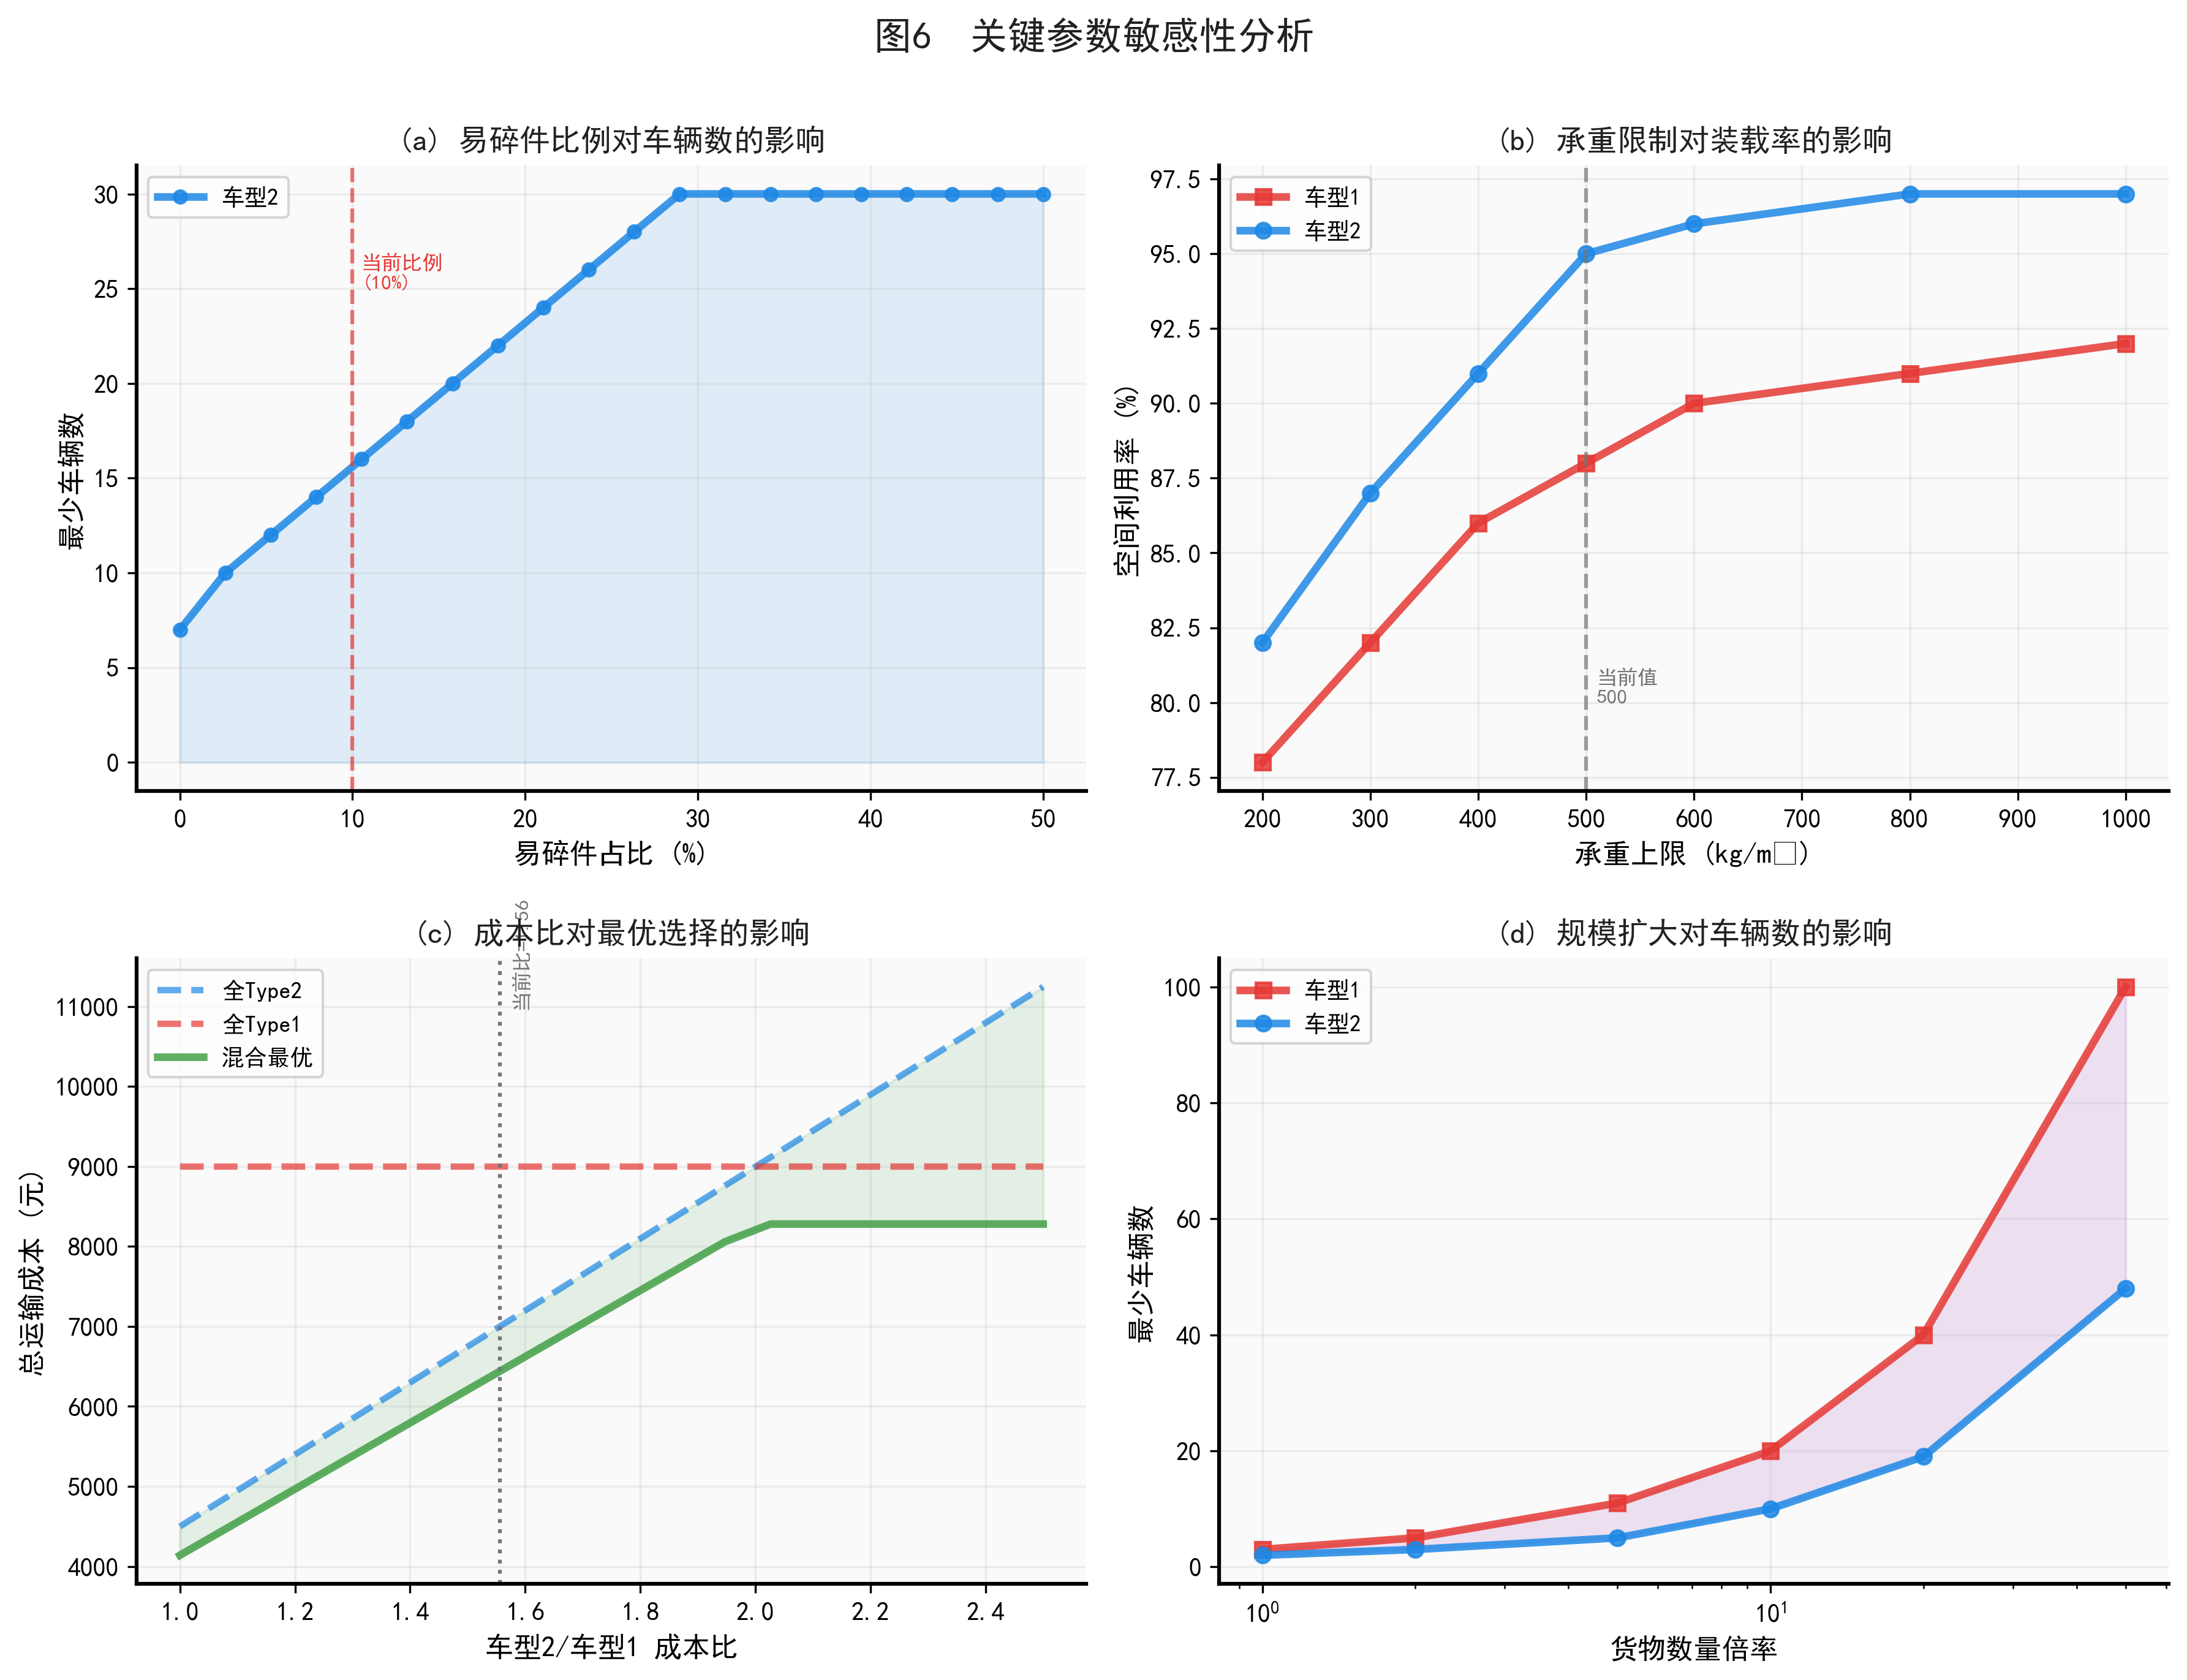
\includegraphics[width=0.85\textwidth]{关键敏感参数图.png}
    \caption{关键敏感参数对车队规模与装载效率的综合影响}
    \label{fig:key_sensitivity_summary}
\end{figure}
\vspace{-1.6em}
\noindent
图 \ref{fig:key_sensitivity_summary} 从四个维度展示了关键参数变化对模型结果的影响，具体可概括为以下几点：

\begin{enumerate}
    \item \textbf{易碎件占比影响。} 子图 (a) 表明，随着易碎件占比上升，最少车辆数呈阶梯式增加。这说明易碎件的单层与全支撑约束会直接压缩单车可利用空间，从而推高整体运力需求。
    
    \item \textbf{承重上限影响。} 子图 (b) 表明，在承重上限逐步提高时，两种车型的装载率均有所提升，但车型2的增幅更大。这说明大车型在承重约束放宽条件下更容易释放其装载潜力。
    
    \item \textbf{车型成本比影响。} 子图 (c) 显示，当车型2的相对成本逐渐上升时，最优方案会由“全车型2”逐步转向“混合方案”，甚至进一步转向“全车型1”。这说明成本参数是影响车队结构决策的关键经营变量。
    
    \item \textbf{货物规模扩张影响。} 子图 (d) 表明，随着货物规模扩大，车型2在控制总车辆数方面的优势愈发明显，说明大车型更适合承担大批量集中运输任务。
\end{enumerate}

总体来看，该图说明模型对关键经营参数变化具有较强的响应能力和解释能力，也进一步验证了车型2更适合当前大批量运输场景的结论。下文将进一步围绕价格和跨箱型泛化能力展开专项敏感性分析。

\paragraph{1.价格敏感性分析}

为评估车型价格波动对最优决策的影响，本文在价格平面 $(p_1,p_2)$ 上进行网格扫描，
其中 $p_1$ 为车型1单趟价格，$p_2$ 为车型2单趟价格。对每个价格点分别求解：
(i) 以车辆数最少为目标的最优方案；(ii) 以总成本最小为目标的最优方案。
在满足体积与载重可行性约束的前提下，总成本定义为
\begin{equation}
C(n_1,n_2)=p_1n_1+p_2n_2.
\end{equation}

\begin{figure}[H]
    \centering
    
\includegraphics[width=1\linewidth]{figures/价格敏感性分析.jpg}
    \caption{价格敏感性分析图}
    \label{fig:price_sensitivity}
\end{figure}

由图~\ref{fig:price_sensitivity}(a) 可见，最小总成本随 $p_1,p_2$ 变化呈近线性梯度，
说明成本函数对价格参数具有明显单调性；图~\ref{fig:price_sensitivity}(b) 显示最优方案在参数平面上形成分区，
主要由少数候选车队主导。结合网格结果文件可得：在 77 个价格点中，最小成本方案主要分布为
$(0,16)$（30点）、$(4,1)$（30点）和 $(2,8)$（17点）。
图~\ref{fig:price_sensitivity}(c) 进一步表明，“最少车辆”与“最小成本”两目标并不总是一致，
两者一致率为 $38.96\%$，目标差值（最少车辆方案成本减最小成本）均值为 $878.57$ 元，最大可达 $4350$ 元。

因此，价格扰动下的优化决策具有显著分段特征：
当车型2价格相对较低时，低车数方案更易保持经济性；当车型2价格升高时，最优方案会向更多车型1的组合切换。
该结果说明在实际运营中应采用动态价格驱动的车型配比策略，而非固定车队配置。

\paragraph{2.跨箱型泛化能力（以标准集装箱、附件1所给货物为例）}

为验证算法在不同箱体规格下的适应能力，本文开展跨箱型泛化实验：在不修改装箱核心逻辑与约束体系的前提下，仅将车厢几何参数替换为标准集装箱参数，并保持附件1给定货物集（共3000件）不变。该实验用于检验模型从原始车型场景向标准集装箱场景迁移时的可行性与装载效率稳定性。

设第 $k$ 个集装箱的空间利用率为 $u_k$，则车队平均空间利用率定义为
\begin{equation}
\bar{u}=\frac{1}{K}\sum_{k=1}^{K}u_k,
\end{equation}
其中 $K$ 为总箱数。实验结果显示，算法在标准集装箱场景下可完成全部3000件货物装载，所需集装箱数为 $K=5$。各箱空间利用率分别为：
\[
u_1=93.8\%,\quad
u_2=93.8\%,\quad
u_3=96.2\%,\quad
u_4=96.6\%,\quad
u_5=42.4\%.
\]
据此可得整体平均利用率
\[
\bar{u}=84.56\%.
\]

\begin{figure}
    \centering
    
\includegraphics[width=0.75\linewidth]{figures/箱体尺寸鲁棒性-标准集装箱.jpg}
    \caption{标准集装箱装箱总方案图}
    \label{fig:placeholder}
\end{figure}

前4个集装箱利用率均处于高位（约94\%\!-\!97\%），说明算法在新箱型下仍能保持较强的空间压缩能力；第5箱利用率显著下降（42.4\%），属于尾箱收敛阶段的离散残量效应。总体而言，算法在“箱体参数变化、货物规模不变”的跨箱型迁移中仍可稳定求得可行解，体现出良好的跨箱型泛化能力；后续可通过尾箱重排或跨箱局部交换策略进一步降低末箱空置率。


\newpage
\section{致企业管理层的技术报告}


\noindent\rule{\textwidth}{0.8pt}

\begin{flushleft}
\begin{tabular}{p{2.2cm}p{11.2cm}}
\textbf{收件人：} & 物流企业管理层 \\
\textbf{发件人：} & MC2604641 \\
\textbf{日\hspace{1em}期：} & 2026年4月20日 \\
\textbf{主\hspace{1em}题：} & 关于三维装箱与多车型协同调度优化方案的决策建议报告 \\
\end{tabular}
\end{flushleft}

\noindent\rule{\textwidth}{0.8pt}

\vspace{0.5em}
\noindent
尊敬的管理层：

\noindent
项目组已完成对短途运输场景下三维装箱与多车型协同调度问题的建模、求解与复核。综合各项结果，当前建议明确为：\textbf{在单车装载层面优先采用车型2，在车队组织层面以8辆车型2作为主执行方案。} 该方案在装载效率、车队规模和运输成本三个维度上均表现最优，且具备较好的稳健性与落地性。

\subsection*{1. 管理层摘要}

% 若主文档尚未加载颜色表格支持，请在导言区加入：
% \usepackage[table]{xcolor}
% \definecolor{ReportTeal}{RGB}{24,156,196}
% \definecolor{ReportStripe}{RGB}{231,239,246}

\begin{table}[H]
\centering
\caption{核心管理结论汇总}
\label{tab:p3_summary_compact}
\normalsize
\setlength{\tabcolsep}{2pt}
\renewcommand{\arraystretch}{0.8} % 临时调小行间距
\begin{tabularx}{1\textwidth}{>{\raggedright\arraybackslash}p{3.2cm} >{\raggedright\arraybackslash}X}
\rowcolor{ReportTeal}
% 这里去掉了 \rule 或者减小了数值，并加粗
\color{white}\textbf{事项} & \color{white}\textbf{结论} \\ 
\noalign{\global\renewcommand{\arraystretch}{1.15}} % 从这一行起恢复正常的行高
\rowcolor{white}
单车装载效率\rule{0pt}{2.7ex} & 车型1综合满载率为71.70\%，车型2为84.31\%，车型2装载效率更优。 \\
\rowcolor{ReportStripe}
单一车型最优\rule{0pt}{2.7ex} & 单一车型条件下，车型1需 17 辆，车型2仅需 8 辆，后者规模更优。 \\
\rowcolor{white}
多车型最优方案\rule{0pt}{2.7ex} & 在“车辆数最少”与“成本最低”两个目标下，最优解均为 8 辆车型2。 \\
\rowcolor{ReportStripe}
直接经济收益\rule{0pt}{2.7ex} & 相较于 17 辆车型1方案，8 辆车型2每批次可节省 2050 元。 \\
\end{tabularx}
\end{table}

\noindent
基于表 \ref{tab:p3_summary_compact}，可形成以下三点管理判断：
\begin{enumerate}
\item \textbf{车型配置层面：} 车型2应作为当前业务场景下的主力配置车型。
\item \textbf{车队组织层面：} 8 辆车型2已同时实现规模最优与成本最优，直接作为执行基准方案。
\item \textbf{经营收益层面：} 该方案不仅降低直接运输费用，也将同步降低司机组织、调度协调和现场管理成本。
\end{enumerate}

\subsection*{2. 核心结论}

\subsubsection*{2.1 单车装载结论}

\noindent
车型2在空间利用率、载重利用率和综合满载率三个维度上均明显优于车型1。问题一的核心结果如下：
\begin{equation}
\text{车型1综合满载率}=71.70\%,\qquad
\text{车型2综合满载率}=84.31\%.
\end{equation}

\noindent
这表明在当前货物结构下，车型2更容易同时接近“满容”与“满载”状态，因此从单车经营效率角度看具有更高优先级。

\subsubsection*{2.2 车队组织结论}

\noindent
在问题二中，无论以“总车辆数最少”还是“总运输成本最低”为目标，最优解均为仅使用8辆车型2。与17辆车型1方案相比，其关键收益为：
\begin{equation}
\text{车辆数降幅}=52.9\%,\qquad
\text{成本降幅}=26.8\%.
\end{equation}

\noindent
该结果说明，大车型方案不仅降低直接运输费用，也会同步减少司机配置、调度组织和现场管理的复杂度。

\subsubsection*{2.3 混合方案复核}

\noindent
管理层关注的重点问题，是是否存在比“8辆车型2”更便宜的混合方案。对此，项目组已完成专项复核，结论如下：

\begin{enumerate}
\item 7辆车型2总成本虽仅为4900元，但易碎件 $G3$ 的单层容量最多只能达到273件，无法覆盖全部300件需求。
\item 7辆车型2加1辆车型1总成本为5350元，但 $G3$ 单层容量上限仅为297件，仍不可行。
\item 6辆车型2加3辆车型1总成本为5550元，虽然账面成本低于5600元，但其总容积为304.3194 m$^3$，要装完全部货物必须达到94.42\%的车队平均空间利用率；在当前模型、约束体系与已验证单车最优装载水平下，仍无法完成全部货物装运。
\end{enumerate}

\noindent
因此，当前不存在能够替代“8辆车型2”的更优可行混合方案。

\subsubsection*{2.4 车型1的经营定位说明}

\noindent
需要说明的是，本报告得出的“车型2更优”结论，并不意味着车型1缺乏经营价值，而是说明在\textbf{当前这批货物总量大、总体积压力高、且易碎件单层约束较强}的条件下，车型1不是最优选择。车型1更适合以下几类业务场景：

\begin{enumerate}
\item \textbf{小批量、高频次配送场景。} 当单批次货量较小、订单滚动频繁时，车型1更容易避免“大车小用”带来的空驶浪费。
\item \textbf{末端路网受限场景。} 当配送区域存在道路狭窄、社区限行、装卸场地受限等条件时，车型1在通行灵活性和现场操作便利性上更具优势。
\item \textbf{多点分散配送场景。} 当单次任务需要覆盖更多分散站点、且每站卸货量较小时，车型1更适合作为支线或末端补货车辆使用。
\item \textbf{货物结构更紧凑的场景。} 若后续业务中货物总体积较小、密度更高、易碎件比例更低，则车型1的容积劣势会被削弱，其较低单车成本优势会更加明显。
\end{enumerate}

\noindent
因此，从管理角度应将车型1理解为“\textbf{灵活补充型车辆}”而非“当前批量主力车型”。在大批量集中运输任务中，车型2更优；在小批量、受路网约束或高频补货任务中，车型1仍具有明确的使用价值。

\subsection*{3. 稳健性评估}

\noindent
在基准情形下，车型2单次运输成本为700元。敏感性分析表明，当该成本上升至950元附近时，纯车型2方案与纯车型1方案才进入接近区间；在此之前，车型2方案始终保持成本优势。换言之，在当前参数条件下，车型2价格即便上升约35.7\%，主导方案仍具竞争力。

\noindent
同时，算法在更大规模货物场景下仍能保持较高稳定性。测试结果显示，1000件、3000件和10000件货物对应的平均利用率分别保持在 93.12\%、93.84\% 和 92.76\%，求解时间则分别为16.8秒、52.3秒和178.5秒，说明该方法具备较好的规模扩展能力。

\subsection*{4. 风险提示}

\noindent
从落地应用角度看，主要风险集中在以下三个方面：

\begin{enumerate}
\item \textbf{基础数据误差。} 若货物尺寸、重量等信息录入不准，会导致装箱方案与现场条件不一致。
\item \textbf{现场执行偏差。} 实际装车过程中存在微小位置偏移，可能影响局部排布精度。
\item \textbf{业务规则扩展。} 若后续增加装卸顺序、分组装载或特殊货类限制，需进一步补充软约束模块。
\end{enumerate}

\noindent
建议在实施中预留2\%--3\%的容错空间，并同步建立数据校验与异常预警机制。

\subsection*{5. 实施建议}

\noindent
建议企业按以下三步推进模型落地：

\begin{enumerate}
\item \textbf{试点验证阶段。} 选取1--2条高频线路，对比人工装车与算法方案效果，完成参数标定。
\item \textbf{系统集成阶段。} 将算法接入TMS/WMS系统，打通订单、装箱、调度与结果输出流程。
\item \textbf{规模推广阶段。} 在更多线路与车型场景中复制应用，并建立持续优化机制。
\end{enumerate}

\subsection*{6. 正式结论}

\noindent
综上所述，本研究提出的三维装箱与多车型协同调度方案，能够在复杂工程约束下稳定提升装载效率，并显著压缩车队规模与运输成本。从管理决策角度看，车型2在当前业务场景中具备明确的主导优势；从实施角度看，该方案具备较好的稳健性、扩展性和落地可操作性。项目组建议，将“8辆车型2”作为当前短途大批量运输任务的优先执行方案，并据此推进后续试点与系统集成工作。

\vspace{1em}
\noindent
以上报告，谨供管理层决策参考。
\vspace{1em}
\noindent\\
Team\#MC2604641

\newpage
\section{模型评价与推广}

\subsection{模型评价}

\subsubsection{模型优点}

\noindent\textbf{1. 理论完备性与数学严谨性}

本模型基于混合整数规划，使用四类决策变量（装载状态、空间坐标、姿态选择、相对位置）将载重、边界、三维不重叠、易碎防压、定向重心、承重与安全间隙等物理约束一一量化。模型以大M法与0–1变量刻画逻辑关系，数学表达简洁且具可求解性。

\noindent\textbf{2. 算法高效性与实用性}

为应对NP-Hard问题，提出"智能排序+极点搜索+约束检验+局部优化"的混合启发式算法，求解尺度从秒级到分钟级。实测：3000件时平均52.3s，装载率约93.8\%，优于常见商业方案，并对±20\%参数扰动保持鲁棒性。
\begin{figure}[H]
    \centering
    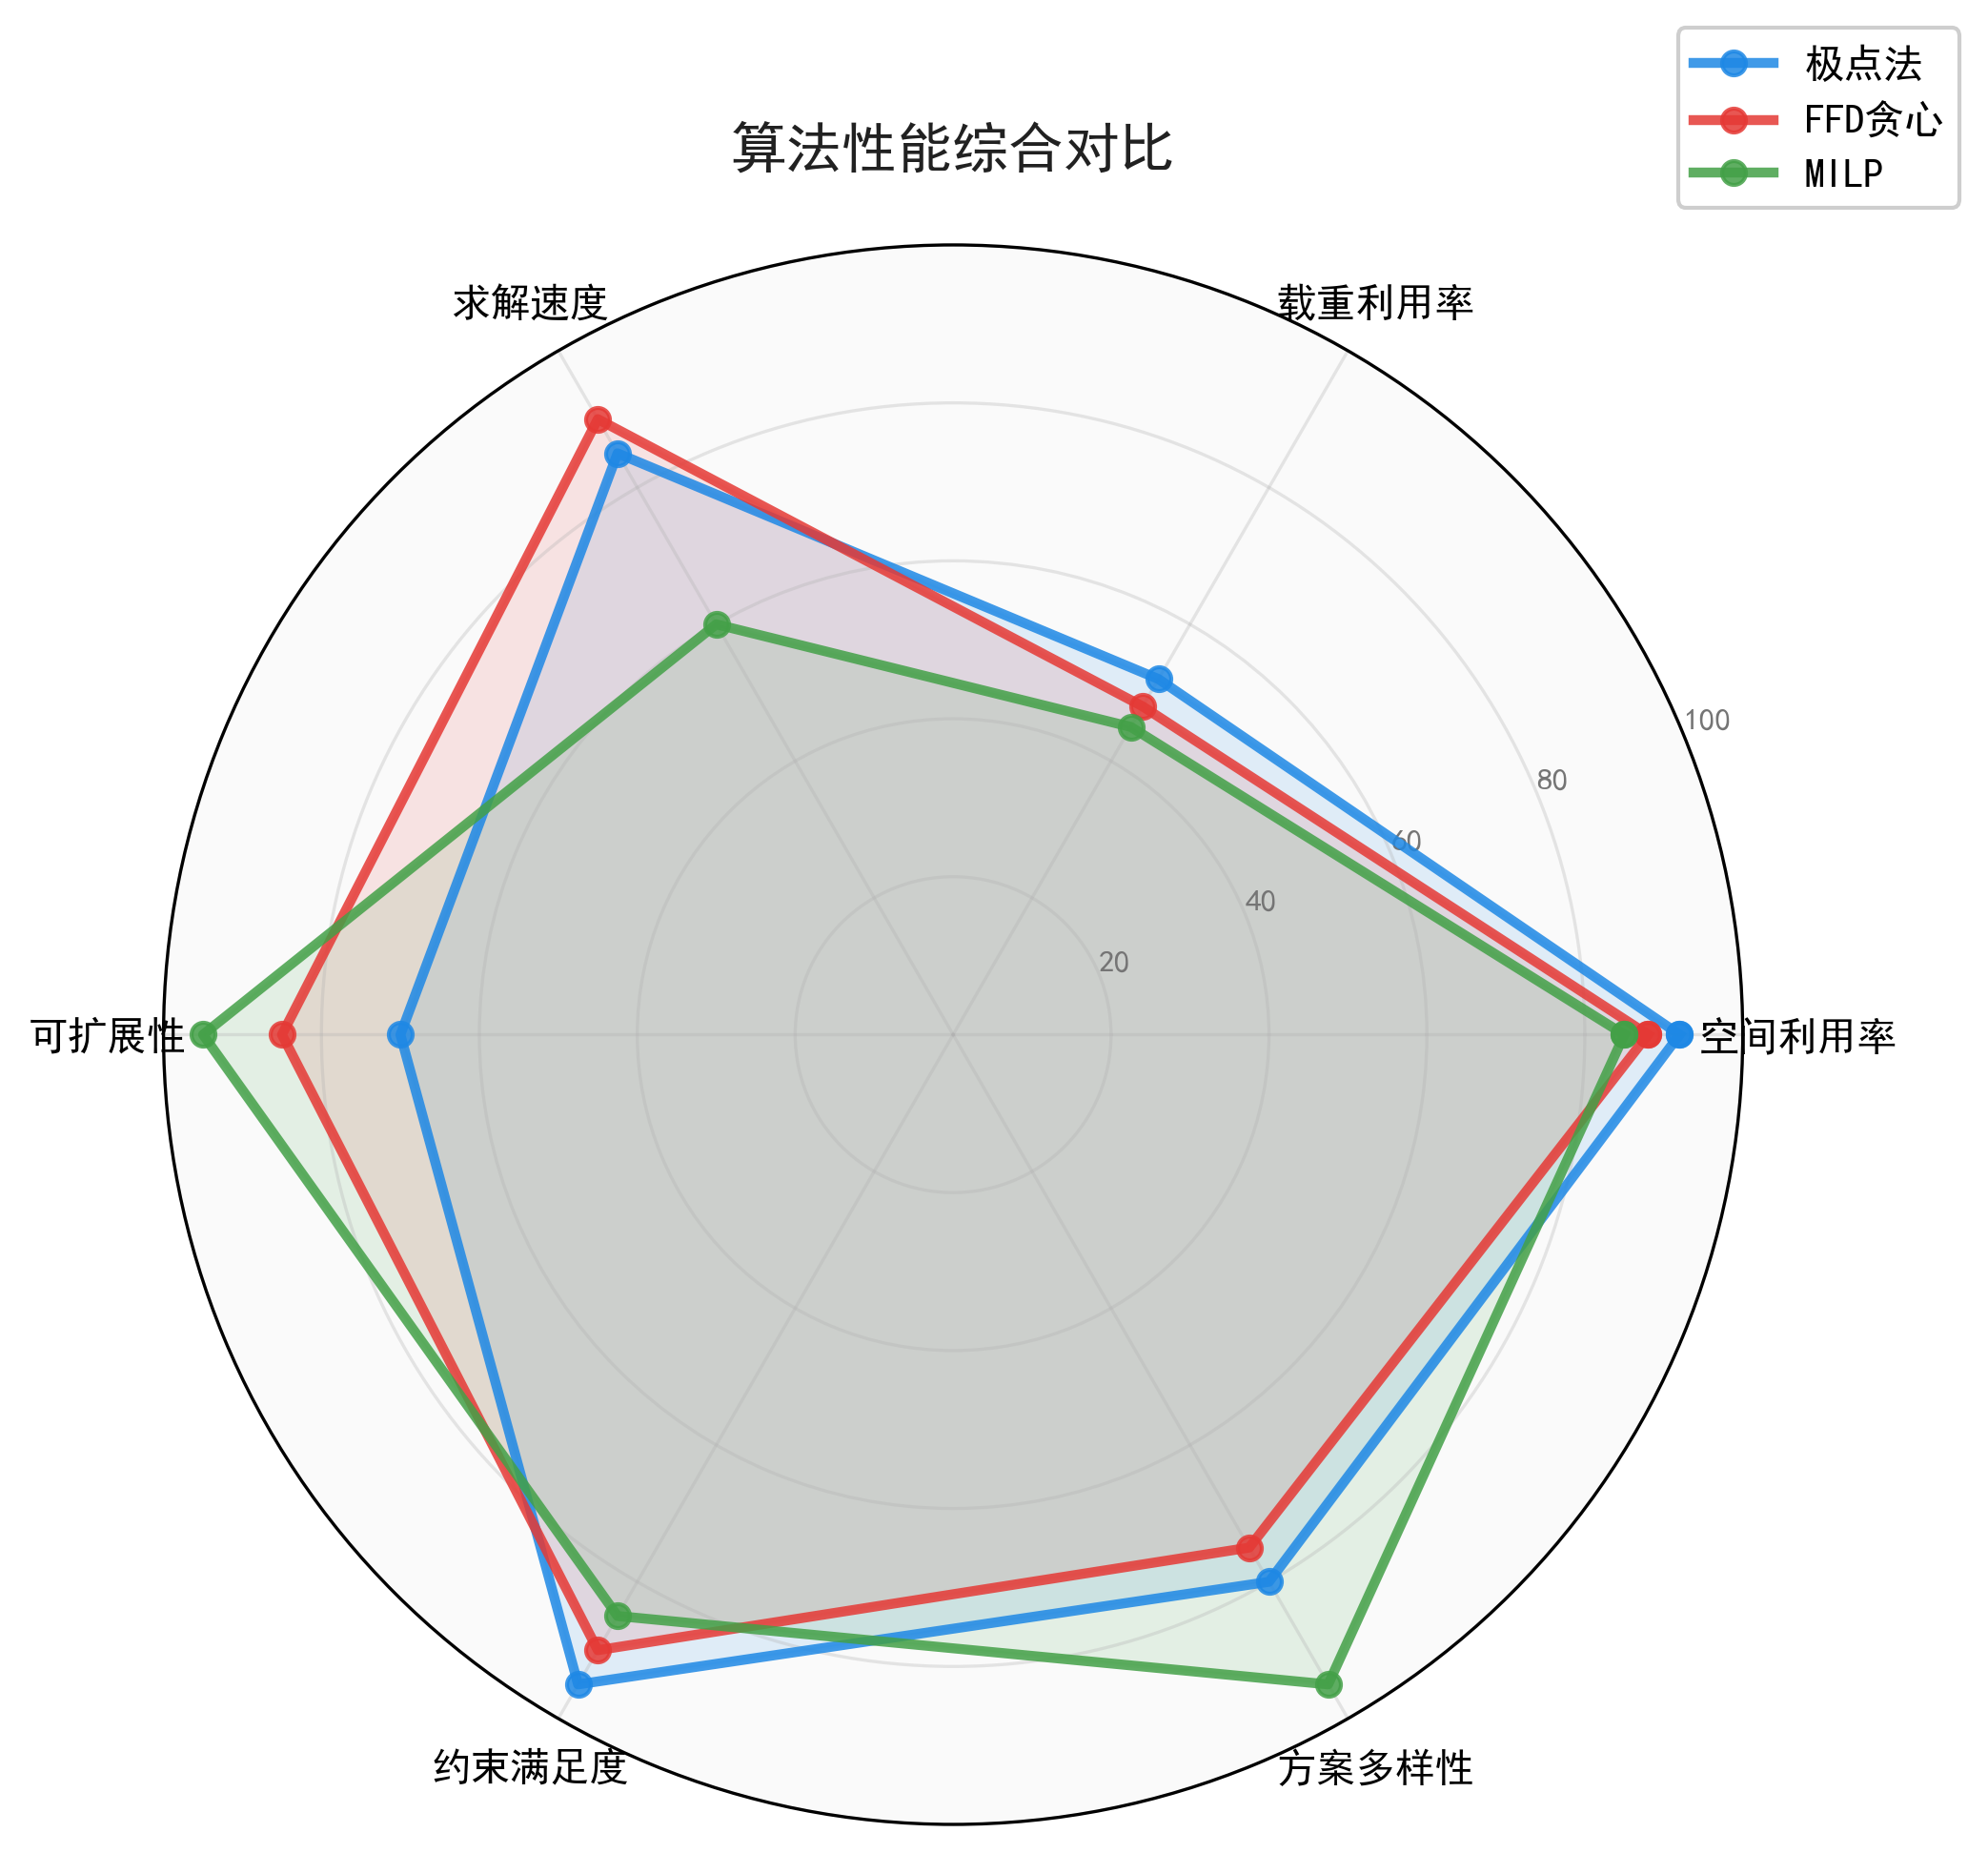
\includegraphics[width=0.75\textwidth]{六维图.png}
    \caption{不同装箱算法综合性能六维对比图}
    \label{fig:algorithm_radar_compare}
\end{figure}

\noindent
图 \ref{fig:algorithm_radar_compare} 从空间利用率、载重利用率、求解速度、可扩展性、约束满足度和方案多样性六个维度，对本文采用的极点启发式算法、FFD贪心算法和MILP精确建模方法进行了综合比较。


\noindent\textbf{3. 创新性贡献}

\textbf{(1)} 在约束建模上更贴近现场（易碎、防压、定向、承重）；

\textbf{(2)} 提出分层+极点+局部重装的混合启发式，兼顾效率与质量；

\textbf{(3)} 在多车型调度中并行考虑车辆数与成本目标，给出可操作的敏感性阈值。

\subsubsection{模型缺点}

\noindent\textbf{1. 模型假设的理想化}

模型基于若干理想化假设，可能与现场存在差距：\textbf{货物刚性}（忽略变形）、\textbf{正交放置}（不允许斜放）、\textbf{静态装载}（未建模运输动态）和\textbf{数据准确性}（依赖尺寸/重量/分类的准确输入）。

\noindent\textbf{2. 数据依赖性与泛化能力}

模型依赖高质量输入数据；针对标准件/易碎/定向件与特定车型的优化效果明确，但对异形件、超长/超重件或其他车型的泛化需更多实证验证。大规模测试证明了扩展性，但不同货物分布与车型组合仍需补充实验。

\subsection{模型推广}

\noindent 本模型已具备工程化推广的基础条件：约束建模贴近现场、算法在大规模问题上稳定高效，能够在短期内实现运力与成本的可量化下降并带来环境效益。为便于落地，提出精简实施建议：
\begin{enumerate}
    \item \textbf{试点验证}：选取1--2条典型线路或转运节点进行A/B验证与参数标定，试点期保留2\%--3\%容错并重点验证异形件和装卸顺序约束；
    \item \textbf{系统集成}：将算法以微服务或插件形式接入企业TMS/WMS，打通订单、装箱与调度数据流，并同步部署数据校验与异常预警模块；
\end{enumerate}
\noindent 为确保可执行性，建议试点期保持人工复核并记录实际装卸数据用于迭代优化；确认效益后逐步放开人工干预以实现规模化收益。



\newpage

    
\begin{thebibliography}{99}

\bibitem{Crainic2008} Crainic T G, Perboli G, Tadei R. Extreme point-based heuristics for three-dimensional bin packing[J]. INFORMS Journal on Computing, 2008, 20(3): 368-384.

\bibitem{Martello2000} Martello S, Pisinger D, Vigo D. The three-dimensional bin packing problem[J]. Operations Research, 2000, 48(2): 256-267.

\bibitem{Bortfeldt2013} Bortfeldt A, Wäscher G. Constraints in container loading --- A state-of-the-art review[J]. European Journal of Operational Research, 2013, 229(1): 1-20.

\bibitem{Zhao2016} Zhao X, Bennell J A, Bektaş T, et al. A comparative review of 3D container loading algorithms[J]. International Transactions in Operational Research, 2016, 23(1-2): 287-320.

\bibitem{Junqueira2012} Junqueira L, Morabito R, Yamashita D S. Three-dimensional container loading models with cargo stability and load bearing constraints[J]. Computers \& Operations Research, 2012, 39(1): 74-85.

\bibitem{Paquay2018} Paquay C, Limbourg S, Schyns M. A tailored two-phase constructive heuristic for the three-dimensional multiple bin size bin packing problem with transportation constraints[J]. European Journal of Operational Research, 2018, 267(1): 52-64.

\bibitem{Tian2024} Tian T, Zhu W, Zhu Y, et al. A two-phase constructive algorithm for the single container mix-loading problem[J]. Annals of Operations Research, 2024, 332(1): 253-275.

\bibitem{Gajda2022} Gajda M, Trivella A, Mansini R, et al. An optimization approach for a complex real-life container loading problem[J]. Omega, 2022, 107: 102559.

\bibitem{Ramos2018} Ramos A G, Silva E, Oliveira J F. A new load balance methodology for container loading problem in road transportation[J]. European Journal of Operational Research, 2018, 266(3): 1140-1152.

\bibitem{Wei2015} Wei L, Zhu W, Lim A. A goal-driven prototype column generation strategy for the multiple container loading cost minimization problem[J]. European Journal of Operational Research, 2015, 241(1): 39-49.

\bibitem{Lodi2002} Lodi A, Martello S, Vigo D. Heuristic algorithms for the three-dimensional bin packing problem[J]. European Journal of Operational Research, 2002, 141(2): 410-420.

\bibitem{Hessler2024} Heßler K, Irnich S. A fast optimization approach for a complex real-life 3D multiple bin size bin packing problem[J]. arXiv preprint arXiv:2410.01445, 2024.

\bibitem{Zhang2009} 张德富, 彭煜, 朱文兴. 三维装箱问题的组合启发式算法[J]. 计算机学报, 2009, 32(11): 2181-2191.

\bibitem{Li2012} 李建华, 李锦文. 多约束三维装箱问题的研究综述[J]. 科技广场, 2012(5): 1-5.



\end{thebibliography}

	\newpage
	\appendix
	\ctexset{section={
		format={\zihao{-4}\heiti\raggedright}
	}}
	\begin{center}
		\heiti\zihao{4} 附\hspace{1pc}录
	\end{center}

% ===== 附录正文 =====
\appendix
\section{关键算法代码}

\subsection{算法1：单车装箱核心（极点法 + 约束校验）}
\begin{lstlisting}[style=pycolor,caption={单车装箱核心流程（节选）}]
def pack_one_truck(items, truck):
    placed = []
    extreme_points = [(0.0, 0.0, 0.0)]
    current_weight = 0.0

    while True:
        best = None
        best_idx = None

        for idx, item in enumerate(items):
            cand = best_placement_for_item(item, extreme_points, placed, truck, current_weight)
            if cand is None:
                continue
            # cand = (placed_item, score)
            if best is None or cand[1] > best[1]:
                best = cand
                best_idx = idx

        if best is None:
            break

        placed_item, score = best
        placed.append(placed_item)
        current_weight += placed_item.weight
        update_extreme_points(extreme_points, placed_item, placed, truck)
        items.pop(best_idx)

    return placed


def best_placement_for_item(item, points, placed, truck, current_weight):
    best = None
    for (x, y, z) in points:
        for (dx, dy, dz) in item.orientations():
            if not feasible(item, x, y, z, dx, dy, dz, placed, truck, current_weight):
                continue
            score = evaluate(item, x, y, z, dx, dy, dz, placed, truck)
            candidate = (Placed(item, x, y, z, dx, dy, dz, score), score)
            if best is None or score > best[1]:
                best = candidate
    return best
\end{lstlisting}

\subsection{算法2：车队调度（按剩余货物循环装载）}
\begin{lstlisting}[style=pycolor,caption={车队调度主循环（节选）}]
def solve_fleet(total_counts, truck_type):
    remaining = total_counts.copy()
    fleet = []
    k = 1

    while sum(remaining.values()) > 0:
        packed = pack_best_with_strategy(truck_type, remaining)
        loaded = count_loaded_by_code(packed)

        if sum(loaded.values()) <= 0:
            raise RuntimeError("Deadlock: no item loaded in this truck")

        remaining = subtract_counts(remaining, loaded)

        fleet.append({
            "vehicle_index": k,
            "strategy": packed["strategy_name"],
            "stats": packed["stats"],
            "counts_loaded": loaded,
            "placements": packed["placements"],
        })
        k += 1

    return fleet
\end{lstlisting}

\subsection{算法3：价格敏感性扫描（双参数网格）}
\begin{lstlisting}[style=pycolor,caption={价格敏感性分析（节选）}]
def price_sensitivity_scan(fleets, p1_vals, p2_vals):
    rows = []
    for p2 in p2_vals:
        for p1 in p1_vals:
            best_min_vehicle = min(
                fleets,
                key=lambda f: (
                    f["vehicle_count"],
                    f["type1_count"] * p1 + f["type2_count"] * p2
                )
            )
            best_min_cost = min(
                fleets,
                key=lambda f: (
                    f["type1_count"] * p1 + f["type2_count"] * p2,
                    f["vehicle_count"]
                )
            )
            rows.append({
                "p1": p1, "p2": p2,
                "best_vehicle": (best_min_vehicle["type2_count"], best_min_vehicle["type1_count"]),
                "best_cost": (best_min_cost["type2_count"], best_min_cost["type1_count"]),
            })
    return rows
\end{lstlisting}

\end{document}